%; whizzy chapter
% -initex iniptex -latex platex -format platex -bibtex jbibtex -fmt fmt
% 以上 whizzytex を使用する場合の設定。

%     Kansai Debian Meeting resources
%     Copyright (C) 2007 Takaya Yamashita
%     Thank you for Tokyo Debian Meeting resources

%     This program is free software; you can redistribute it and/or modify
%     it under the terms of the GNU General Public License as published by
%     the Free Software Foundation; either version 2 of the License, or
%     (at your option) any later version.

%     This program is distributed in the hope that it will be useful,
%     but WITHOUT ANY WARRANTY; without even the implied warranty of
%     MERCHANTABILITY or FITNESS FOR A PARTICULAR PURPOSE.  See the
%     GNU General Public License for more details.

%     You should have received a copy of the GNU General Public License
%     along with this program; if not, write to the Free Software
%     Foundation, Inc., 51 Franklin St, Fifth Floor, Boston, MA  02110-1301 USA

%  preview (shell-command (concat "evince " (replace-regexp-in-string "tex$" "pdf"(buffer-file-name)) "&"))
% 画像ファイルを処理するためにはebbを利用してboundingboxを作成。
%(shell-command "cd image200708; ebb *.png")

%%ここからヘッダ開始。

\documentclass[mingoth,a4paper]{jsarticle}
\usepackage{kansaimonthlyreport}
\usepackage[dvips]{xy}
\usepackage{ascmac}

% 日付を定義する、毎月変わります。
\newcommand{\debmtgyear}{2010}
\newcommand{\debmtgdate}{28}
\newcommand{\debmtgmonth}{02}
\newcommand{\debmtgnumber}{32}

\begin{document}

\begin{titlepage}

% 毎月変更する部分、本文の末尾も修正することをわすれずに

 第\debmtgnumber{}回 関西 Debian 勉強会資料

\vspace{2cm}

\begin{center}
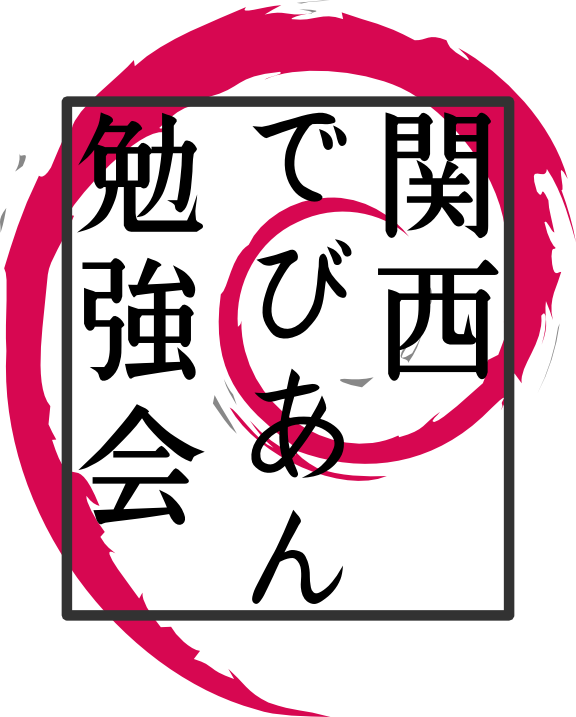
\includegraphics{image200802/kansaidebianlogo.png}
\end{center}

\begin{flushright}
\hfill{}関西 Debian 勉強会担当者 佐々木・倉敷・のがた \\
\hfill{}\debmtgyear{}年\debmtgmonth{}月\debmtgdate{}日
\end{flushright}

\thispagestyle{empty}
\end{titlepage}

\dancersection{Introduction}{Debian JP}

\subsection*{}%ロゴ用のスペース稼ぎ
 
関西 Debian 勉強会はDebian GNU/Linux のさまざまなトピック(新しいパッケー
ジ、Debian 特有の機能の仕組、Debian 界隈で起こった出来事、などなど)に
ついて話し合う会です。

目的として次の三つを考えています。
\begin{itemize}
      \item MLや掲示板ではなく、直接顔を合わせる事での情報交換の促進
      \item 定期的に集まれる場所
      \item 資料の作成
\end{itemize}

それでは、楽しい一時をお楽しみ下さい。

\clearpage

\begin{minipage}[b]{0.2\hsize}
 {\rotatebox{90}{\fontsize{80}{80}
{\gt 関西デビアン勉強会}}}
\end{minipage}
\begin{minipage}[b]{0.8\hsize}
\hrule
\vspace{2mm}
\hrule
\setcounter{tocdepth}{1}
\tableofcontents
\vspace{2mm}
\hrule
\end{minipage}

\dancersection{事前課題}{のがたじゅん}

関西でも事前課題を始めました。2月の課題は2点のどちらかを選んで答えてもら
いました。

\begin{itemize}
 \item Debianを使ったサーバーを管理している人は、セキュリティについてど
       うしているか、どこに気をつけているか教えてください。
 \item 今回から新しく使うDebian勉強会予約管理システムについての感想を教
       えてください。
\end{itemize}

\begin{prework*}{ 名村 知弘 }

    個人用途で web サーバを使用しています。
    セキュリティについてはほとんど考えていないダメ管理人です。
    一応以下のような、なんちゃって対策をしています。
    \begin{enumerate}
          \item ルータ内にサーバを設置する。
          \item HTTPは80/8080ではないオリジナルポートを使用する。
          \item HTTPSは443を使用しているが、クライアント認証する。 
        たまにログを見て、自分しかアクセスしていないことで安心してます。
    \end{enumerate}
\end{prework*}

\begin{prework*}{ 佐々木洋平 }
    サーバ管理について:
    \begin{itemize}
          \item apache2 + qmail + 自作のユーザ管理 cgi でサーバを
        動かしてます。
          \item iptables で必要なポート以外は閉じています。
          \item なるべく最小限構成にするようにしています。定期的に
        deborphan などを駆使して不要なパッケージを purge してます。
          \item 最近 syn\_flood 受けていて困ってますね。どうしよ。
    \end{itemize}
    勉強会システム:
    \begin{itemize}
          \item google アカウント以外での登録もできるのかしら?
        \footnote{上川注:現在できません}
          \item google アカウントとは別に名前を登録できると良いですね
        -> gmail のアカウントはあんまり知られたくないもんで.
        今回のでバレバレですな(笑) 
        \footnote{上川注:
          アカウント名ではなく「名前(提出課題一覧・出席確認のための名前です、本人
          確認できるようにしてください)」と書いてある部分に記
          述した名前で登録されます。アカウント名はイベントの管理者にしか
          バレないはずです。}
    \end{itemize}
\end{prework*}

\begin{prework*}{ lurdan }
    アップデートに追従する、追従できるような構成にしておく、余計なもの
    は入れない動かさない、といったところです。
\end{prework*}

\begin{prework*}{ tosihisa }
    \begin{itemize}
          \item むやみにサーバを立てない。1台サーバを立てる毎に眠れない
        日が増える。
          \item サーバダウン時の緊急連絡先を作る。
          \item 一人で管理しない。台数にもよるが、1台のサーバ維持に3名
        は見た方が良い。
          \item 「裏口」を作らない。
          \item 自分だけに特権を作らない。自分も他の人も同じ。root だけが違う。
          \item 人から信頼を得る事。どれだけ Debian の事が詳しくても、
        信頼が得られなければ、人のパスワード、メールデータは預けられな
        い。信頼されて、初めてサーバ管理者である事を肝に銘じる
        事。Debian はその後。
    \end{itemize}
\end{prework*}

\begin{prework*}{ 山下康成@京都府向日市 }
    15 分ほどしゃべっていいでしょうか?\footnote{オーケーです(佐々木)}
\end{prework*}

\begin{prework*}{ 永田昭雄 }

    今回から新しく使うDebian勉強会予約管理システムについての感想:

    google accoutsに登録してすぐにこのページがでてきたのには、びっくりしまし
    た。今までよりもわかりやすいようでいいと思います。
    
\end{prework*}


\begin{prework*}{ 村松耕司 }

    Debian勉強会予約管理システムについての感想:
    
    シンプルなインターフェースで使いやすいと思いました。
    今回のソースについての話も楽しみにしています。
    
\end{prework*}

\begin{prework*}{ のがたじゅん }

    Debianサーバーで気をつけているところは、以前はサーバー兼ルーターだっ
    たのでiptablesでガチガチにルールを書いたりしていましたが、ルーター
    は分けてサーバーのみ、サービスはwebぐらいしかないので以前ほどは気を
    遣っていません。
    
    \begin{itemize}
          \item 基本的には何もいれてません。(インストール時のtaskselも
        何も選ばずaptitudeで後から入れてます)
          \item sshはポートを変えて鍵認証のみ。
          \item logwatchでlogメールを飛ばしてながし読み。
          \item rkhunter入れてます(たまに誤検出があるのがちょっと…)
          \item cron-aptで更新されたパッケージをダウンロードしてます(アッ
        プデートはどう変わったのかを見てから手動です)
          \item バックアップにはrdiff-backup使ってます。
    \end{itemize}

\end{prework*}

\begin{prework*}{ 原口 秀人 }
    
    \begin{itemize}
          \item TCP WrappersでSSH接続のIP制限
          \item iptablesによるポート制限
          \item ファイルの所有者:ユーザー:パーミッションの適切な設定
          \item JPCERT/CCのサイトをRSSで購読
          \item その他、DebianMLでのセキュリティ情報の確認など。
    \end{itemize}
    
\end{prework*}

\begin{prework*}{ 木下敏夫 }

    こまめに aptitude update している他、ssh のポートを標準外にすること
    でsshへのアタックをされにくくしたりサーバー設置時に余分なパッケージ
    を読み込まない等して設置時から気を付けています。
    
\end{prework*}

\begin{prework*}{ 城(じょう)タカヒロ }
    
    サーバの管理を小規模ながらやらせていただいています。セキュリティについて
    ですが、以下の点を実地(未実地も含)しています。
    
    初期セットアップでは
    \begin{itemize}
          \item 標準パッケージの調整
        \begin{itemize}
              \item - exim4\*,portmap\*,inetd関係
              \item + openssh-server, sudo,ntpdate, php5-cli (swatch, arpwatch)
        \end{itemize}
          \item 不要ユーザ・持ち物の削除
          \item iptablesによるロギング(hashlimitによる制御)
          \item マウントオプションの調整(出来ていない)
          \item logrotate設定の変更(延長)
          \item ホスト鍵のバックアップ
    \end{itemize}
    
    運用
    \begin{itemize}
          \item 以下のレポートを毎日メールしています
        \begin{enumerate}
              \item システムの稼動情報
              \item ログイン履歴
              \item ファイル改変履歴
              \item DISK利用容量
              \item ネットワーク転送量
              \item SAMBA統計情報
              \item Apache統計情報
              \item ファイル改変内容報告
              \item DHCP割当状態報告
              \item ARP情報を添付
            →毎日0時半に昨日の状態を関係者にメール
        \end{enumerate}
          \item ログは別のホストにも投げています
          \item SWATCHによる通知(これはビジネスレベルでの警告が主)
    \end{itemize}
    
    アプリケーション
    \begin{itemize}
          \item sshdのパラメータ調整
          \item DNSのJail化
    \end{itemize}
    
    初めて参加させていただきます、よろしくお願いいたします。
    
\end{prework*}


\begin{prework*}{ dictoss(杉本 典充) }
    
    $\circ$サーバ管理で気をつけていること
    \begin{itemize}
          \item サーバには限定したポートのパケットのみを届くようにす
        る。(私の場合、個人サーバで負荷が低いためDSUのポートフォワード
        機能を使用しています。)
          \item top、vmstat、df等でCPU、メモリ、ディスクに異常に負荷が
        かかっていないかチェックする。
          \item psで怪しいプロセスがいないか確認する。
          \item ログを定期的に見る。
          \item 影響のありそうなセキュリティパッチは早めにインストールする。
          \item 動かすアプリケーションの脆弱性のチェック(これは勉強中)
    \end{itemize}
    
\end{prework*}

\begin{prework*}{ 河田鉄太郎 }

    \begin{itemize}
          \item debian-security-announce を購読する
          \item debian の流儀にあわせる
          \item あんまりいじらないけどよく見る
          \item 必要ないもの以外は入れない
    \end{itemize}
    
\end{prework*}

\begin{prework*}{ IPv6waterstar }
    
    セキュリティに関しては基本的にiptablesで対応しています。ただ、メー
    ルサーバとかは直接、外部のメールと接するので、ウィルス対策とし
    てClamavを使ってます。Webサーバとかは現在検討中。それと、特にログに
    ついては毎日、目を通しています。
\end{prework*}


\dancersection{最近のDebian関係のイベント報告}{Debian JP}

\subsection{前回の関西 Debian 勉強会}

川江さんによる「Xenで作ろう自宅の仮想サーバ」の発表と、倉敷さん司会によ
る2009年を振り返りつつ、2010年のネタ出しをした「2010年の関西Debian勉強会を
企画しよう」がありました。

2009年の関西Debianを振り返っての反省点は
\begin{itemize}
 \item Debianから外れるネタが多かったので、ちょっと方向修正。
 \item 京都や神戸で開催したとき新しい人が来たので、たまには場所を変えてみる。
\end{itemize}
でした. 

2010年にしたいネタとしては
\begin{itemize}
 \item Debian Alternative Systemの話。
 \item Gitの話(使い始めのあたりぐらいのレベルで)
 \item 勉強会リポジトリの話(Gitと関連して)
 \item パッケージ作成の話しをもう一度(dh7とかcdbsとの比較とか)
 \item ubuntuとの違い(いくやさんとか呼ぶ?)
 \item BTSハンズオン
\end{itemize}
などが提案されています. 


\begin{figure}[h]
 \begin{center}
 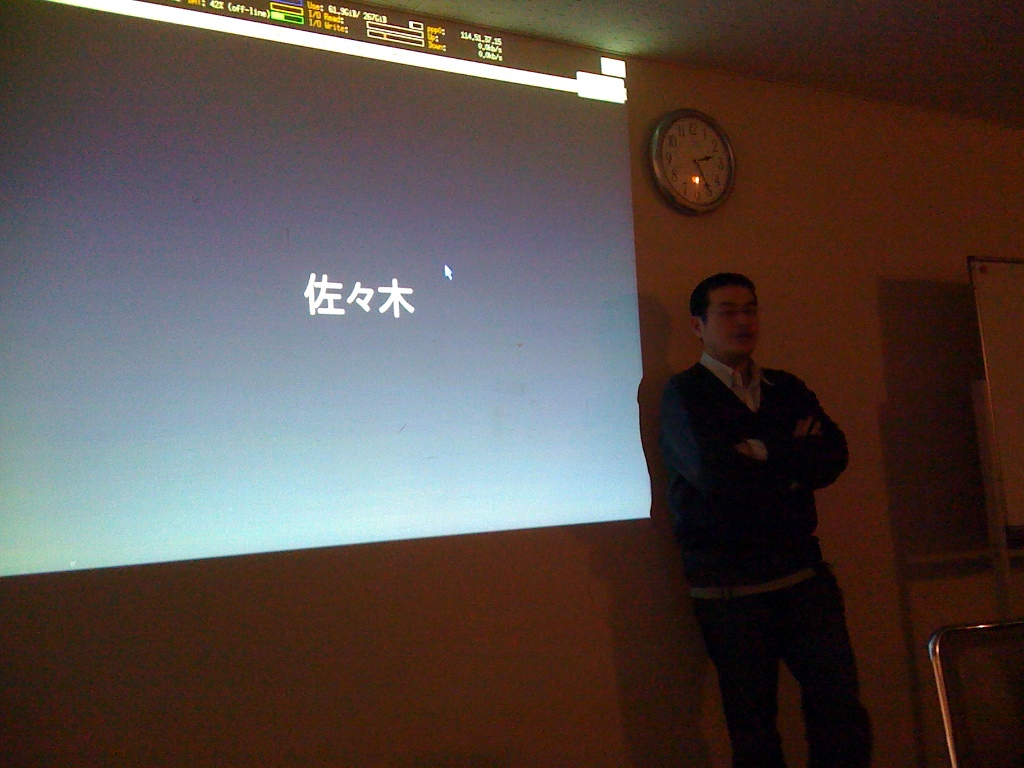
\includegraphics[width=4cm]{image201002/kansaimeeting1.jpg}
 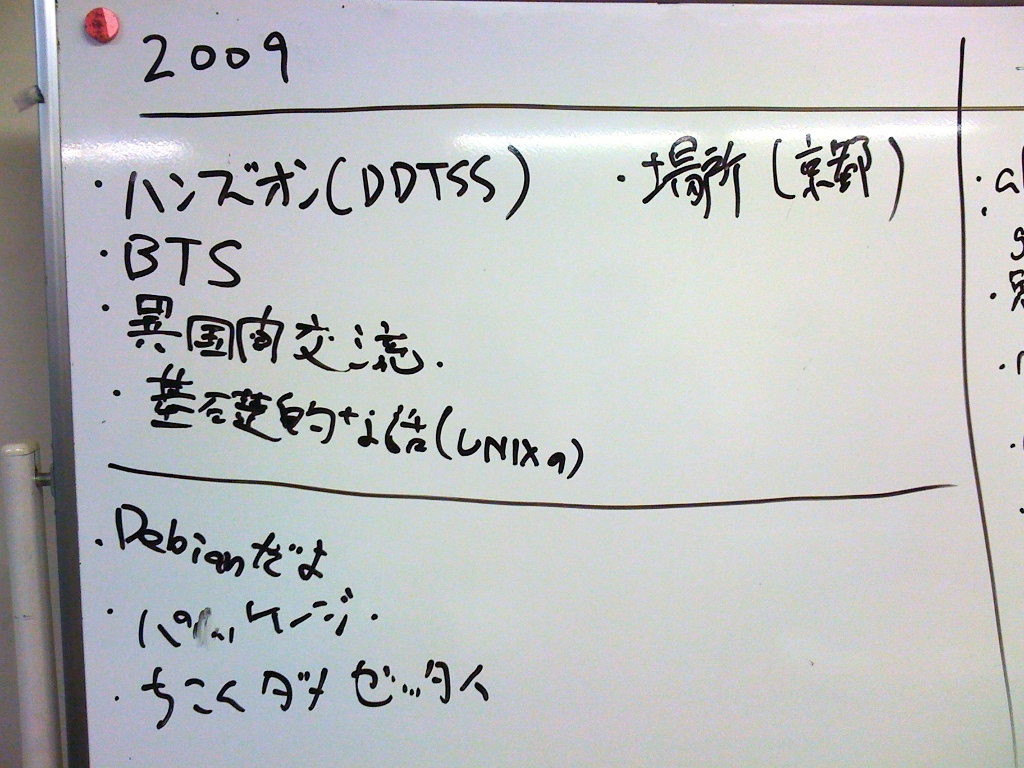
\includegraphics[width=4cm]{image201002/kansaimeeting2.jpg}
 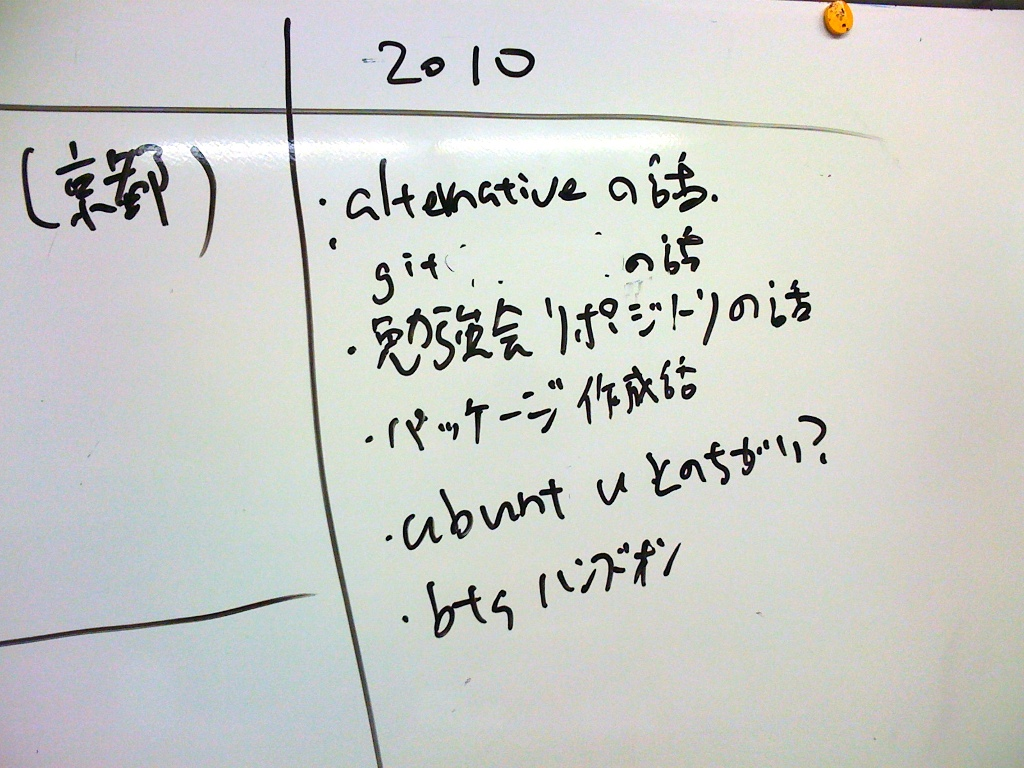
\includegraphics[width=4cm]{image201002/kansaimeeting3.jpg}
 \caption{勉強会の様子とまとめホワイトボード}
 \end{center}
\end{figure}

\subsection{第61回 東京エリア Debian 勉強会「でびあん温泉@木更津」}

2月20日と21日にわたり木更津工業高等専門学校 情報工学科の方々の協力で
「でびあん温泉@木更津」が開かれました。mkouhei さんのレポートによれ
ば, 表のテーマは「関数型言語」「温泉」であったけれども, 開催して気がつ
いた真のテーマは「縁」だそうです.
\begin{screen}
    \begin{quote}
        やまねさんが事前課題回答、セッションでびあん勉強会を通じた縁以
        外に、関数型言語やニューラルネットワークといった興味のある話題
        を通じた縁、でびあんーうせのを通じた縁、Debian と Ubuntu という
        ディストリビューションを通じた縁、一昨年の Debian 温泉を通じた
        縁、などなど色々ありますが、特に昨年秋の OSC で「東京都心だけで
        なく木更津などの郊外でも開催してほしい」と坂口さんが要望を出し、
        現地の幹事として実際に動いてくださった、というのが一番大きな縁
        じゃないかと思います。
    \end{quote}
    \begin{flushright}
        -- 第61回東京エリアDebian勉強会&第2回Debian温泉:
        \url{http://d.hatena.ne.jp/mkouhei/20100222/1266808155}
    \end{flushright}
\end{screen}
今回の前田さんの発表も「縁」からです. 大事にしたいですね.


\subsection{OSC 2010 Tokyo/Spring}

2/26-27(一昨日と昨日) には オープンソースカンファレンス 2010
Tokyo/Spring が開催されていました. 
東京 Debian 勉強会もブースとセッションで参加しています. 
参加者\&運営側によるレポートは次月の資料を期待してください.

また, 3/13 には OSC 2010 Kobe があり, 
関西 Debian 勉強会も参加する予定です. 
皆様よろしく御願いします.


\dancersection{PythonもGoogle App Engineも知らない人が「Debian勉強会予約管理システム」のソースを見てみたよ}{のがたじゅん}

\subsection{はじめに}

結論をいうと当初の目標「OpenIDよるログインの実装」はできませんでした。

\subsection{とりあえずやったことを書いてみる}

それはさておき、まったく何もしなかったわけではないので、この一ヶ月やって
みたことを書きます。

\subsubsection{ソースはどこ}

「見る」と言ったからからには、「Debian勉強会予約管理システム」のソースは
どこかと探してみると、勉強会リポジトリのutils/gae/ディレクトリに置いてあ
ります。

自分は関西Debianの資料を作るので手元にリポジトリはありましたが、見てみた
いなと思った人は勉強会リポジトリをgit cloneしてください。

\begin{commandline}
 $ git clone git://git.debian.org/git/tokyodebian/monthly-report.git
\end{commandline}

\subsubsection{Google App Engineとは何者?}

Google App Engineが何者かわからないので公式ページを見てみた。

\begin{itemize}
 \item \url{http://code.google.com/intl/ja/appengine/}
\end{itemize}

ええっと。ざっくり言うとWebアプリに必要なサーバーからデータベース、開発環
境までまるっと一式無償で使わせてくれるGoogleのサービスという認識でおk?

フレームワークにはJavaとPythonを使ったものがあって、勉強会予約システムは
Pythonを使ってる。

公式ページの頭のところに開発を始める人のためのクイックガイドが書いてある
ので、それに沿って始めればいいのか。

\subsubsection{クイックスタートの順番にしてみた}

まずクイックスタート1番目には、「App Engine カウントを登録します」と書い
てあるけど、今のところ公開するつもりはないので飛ばして、「Google App
Engine SDK for Python」の「 Linux/その他のプラットフォーム」のSDKをダウン
ロード。

\begin{itemize}
 \item \url{http://googleappengine.googlecode.com/files/google_appengine_1.3.1.zip}
\end{itemize}

アーカイブを展開して、クイックスタートを見ると「スタートガイドを参照しま
す」だそうなので読んでみた。
\begin{itemize}
 \item \url{http://code.google.com/intl/ja/appengine/docs/python/gettingstarted/}
\end{itemize}

「概要」を見るとスタートガイドを読むと一通り作れるように説明してあるので、
まず読んでみる。

「開発環境」の説明を読むと、SDKにあるdev\_appserver.pyを使うとローカルで動か
すこともできるのか。
PythonはDebianだと頼まずとも入っているので、特にインストールする必要はな
し。ライブラリ関係も書いてないので、飛ばしてもいいかな。

Pythonといえばインデントなので、エディタ必須だけど開発に使う環境はどうし
たらいいだろう。試しにemacsでpython-mode.el、pymacs、ipythonの環境を作ろ
うとしたけど、どうもしっくりこない。

いい機会なので、geany、gedit、kate、scribesなどエディタをとっかえひっかえ
試してみたけど、geditのpythonコンソール、コードスニペット、外部のツール、
埋め込み式の端末プラグインを有効にすると、タブ補完も効くし、ターミナルや
Pythonコンソールもあるので試しながら使えるので、なかなかいい感じ。灯台下
暗しとはこのことか。

\subsubsection{世界のみなさんこんにちは!}
スタートガイドの「Hello,world!」からコードが出てきた。

まず最初はCGIを作るとき一番最初に説明するようなHTTPヘッダとメッセージを出
力するhelloworld.pyともう一つ。Google App Engineならではの設定ファイルを
YAMLで書いて置かないと、使えないそうな。

アプリケーションのテストはディレクトリを指定してSDKについてた
dev\_appserver.pyを実行。

\begin{commandline}
 $ google_appengine/dev_appserver.py helloworld/
\end{commandline}

ブラウザで \url{http://localhost:8080/} を開くとアプリケーションが使える
と。

Webサーバーを起動したままコードを書き換えられるのは、RubyのSinatraみたい。

\subsubsection{webappフレームワークがわからない}

\begin{quote}
App Engine には、シンプルな独自の Web アプリケーション フレームワークが用意されています。これが webapp です。

webapp フレームワークの使用 - Google App Engine - Google Code:
 \url{http://code.google.com/intl/ja/appengine/docs/python/gettingstarted/usingwebapp.html}より。

\end{quote}
 

ええ!シンプルというけれど、なんの説明もなくいきなり!

すいません。ここでわからなくなり、みんなのPythonを買って読んだりしていた
ら時間切れになりました。

予約システムのdebianmeeting.pyなども見たところ、チュートリアルから派生し
た感じのようなのですが、似たような事をしているということはチュートリアル
の意味がわからなければ、予約システムもわからないということで…。すいませ
ん。


\subsection{これから}


\subsubsection{予約システムで解決したいところ}


\begin{itemize}
 \item OpenIDでログインしたい \\
        今回、解決したい目標でもあったことですが、勉強会に参加するために、
       わざわざGoogleアカウントを取らなければいけないのは参加者の利便性を
       そこなうし、Googleのプラットフォーム依存は自由ではないので早めに
       解決したいですね。
       
        幸い、Google App EngineのアプリケーションギャラリーにOpenIDのサ
       ンプル
       \footnote{\url{http://appgallery.appspot.com/results?q=openid}} が
       あるので、それを見ながら、なんとか実装できるようになりたいと思って
       ます。\\

 \item トップページから予約ページに飛びたい \\
       予約システムのトップページで、参加者がEventIDを入力するようになっ
       ていますが、EventIDが長すぎるので、おそらく誰も使っていないと思わ
       れます。
       EventIDを入力しなくとも、トップページに直近のイベントのリンクがあ
       ればEventIDを入力しなくて済むので、これも解決したいですね。\\

 \item テンプレートのHTMLをきれいにしたい \\
       今はdivタグでくるんだりして、あらっぽいので直したいですね。
\end{itemize}

事前課題でも書いていた人がいましたが、シンプルであるのはいいところだと思
うので、シンプルさをうしなわないように、よりよくしたいですね。

\begin{thebibliography}{99}
 \bibitem{tokyo61}
         第61回東京エリアDebian勉強会 \\
         東京エリアDebian勉強会予約システムの構想: 上川 純一 \\
         \url{http://tokyodebian.alioth.debian.org/pdf/debianmeetingresume201002.pdf}
\end{thebibliography}


\dancersection{今後の予定}{Debian JP}

\subsection{オープンソースカンファレンス Kansai @ Kobe 2010}

2010年3月13日土曜日にJR神戸駅すぐそばの神戸市産業振興センターにて、
オープンソースカンファレンス Kansai @ Kobe 2010が開催されます。
関西Debian勉強会は、OSC2010Kobeに参加します。

\subsection{次々回の関西Debian勉強会}

次々回、2010年4月の関西Debian勉強会は 4月25日におこなう予定です。

% 冊子にするために、4の倍数にする必要がある。
% そのための調整
\dancersection{メモ}{}
\mbox{}\newpage

\printindex
 \cleartooddpage

 \begin{minipage}[b]{0.2\hsize}
  \rotatebox{90}{\fontsize{80}{80} {\gt 関西デビアン勉強会} }
 \end{minipage}
 \begin{minipage}[b]{0.8\hsize}

 \vspace*{15cm}
 \rule{\hsize}{1mm}
 \vspace{2mm}
 
\includegraphics[width=2cm]{image200502/openlogo-nd.eps}
 \noindent \Large \bf Debian 勉強会資料\\ \\
 \noindent \normalfont \debmtgyear{}年\debmtgmonth{}月\debmtgdate{}日 \hspace{5mm}  初版第1刷発行\\
 \noindent \normalfont 関西 Debian 勉強会 (編集・印刷・発行)\\
 \rule{\hsize}{1mm}
 \end{minipage}

\end{document}
